\renewcommand{\rmdefault}{lmss} 
\renewcommand{\sfdefault}{lmss}

\documentclass{article}

\usepackage{graphicx} %inserting graphics
\usepackage{float} %positioning image
\usepackage{subcaption} % allow multiple figures
\usepackage{setspace} % alter spacing
\usepackage[justification=raggedright]{caption}
\usepackage[left=2cm,right=2cm,top=2cm,bottom=2cm]{geometry}

\title{HPC Week Exercise Answers}
\author{Katie Bickerton}

\begin{document}

\section*{HPC Exercise Written Answers}


\paragraph{Question 8:}\

\noindent \newline In the simulation, the species richness drops to a value close to 1, indicating a dominant species Figure \ref{fig:qu8}a. When the simulation is run using 100 different scenarios, Figure \ref{fig:qu8}b, each converges to a low value of species richness, indicating that a highly diverse system is likely to be dominated by several key species, indicating that despite species abundances being equal intially, it is very unlikely they will remain this way.  \newline

	\begin{figure}[H]
			\centering %centre figure
			\textbf{Neutral model simulation over 200 generations}\par\medskip
			% set line width manually
			\begin{subfigure}[t]{0.49\linewidth}
				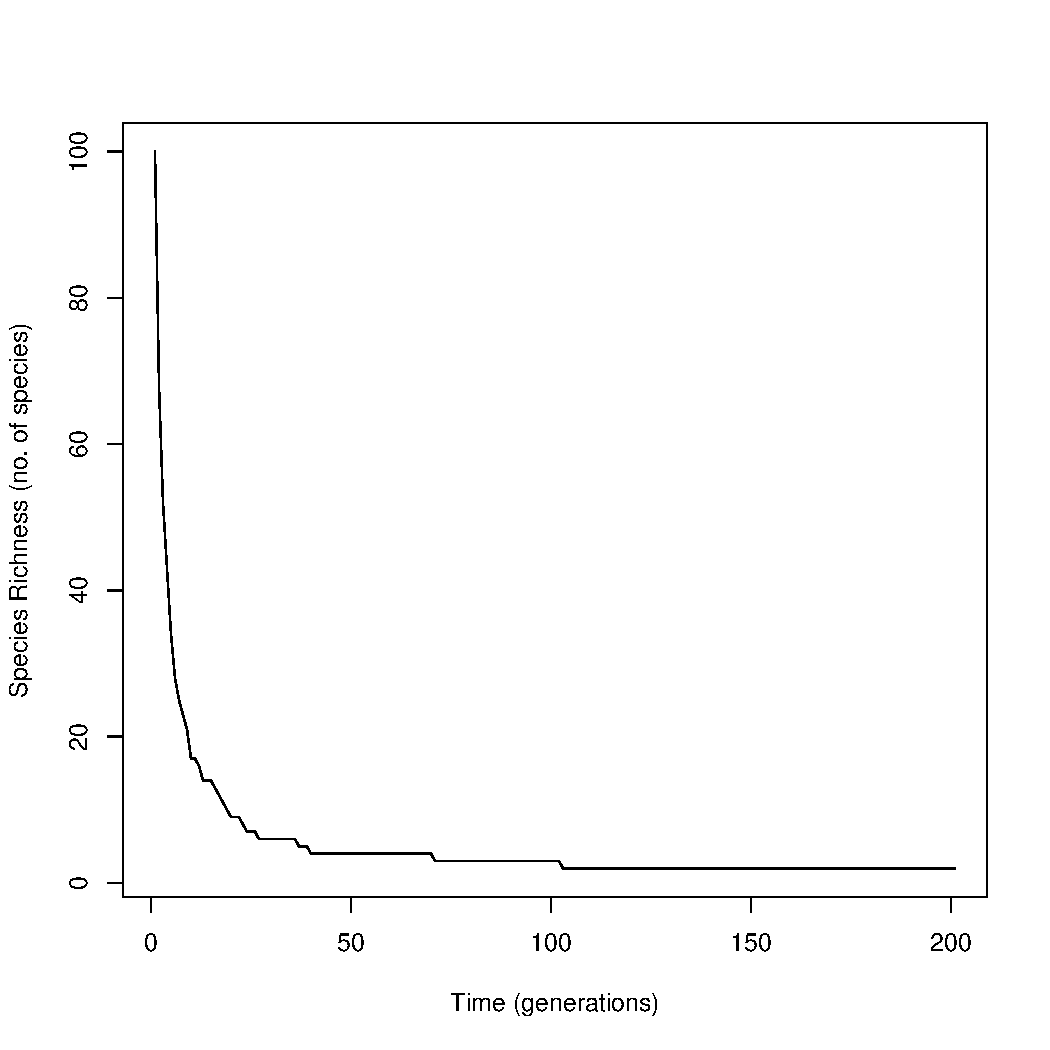
\includegraphics[width=\linewidth]{../Results/time_series.pdf}
				\caption{}
			\end{subfigure}
			\begin{subfigure}[t]{0.49\linewidth}
				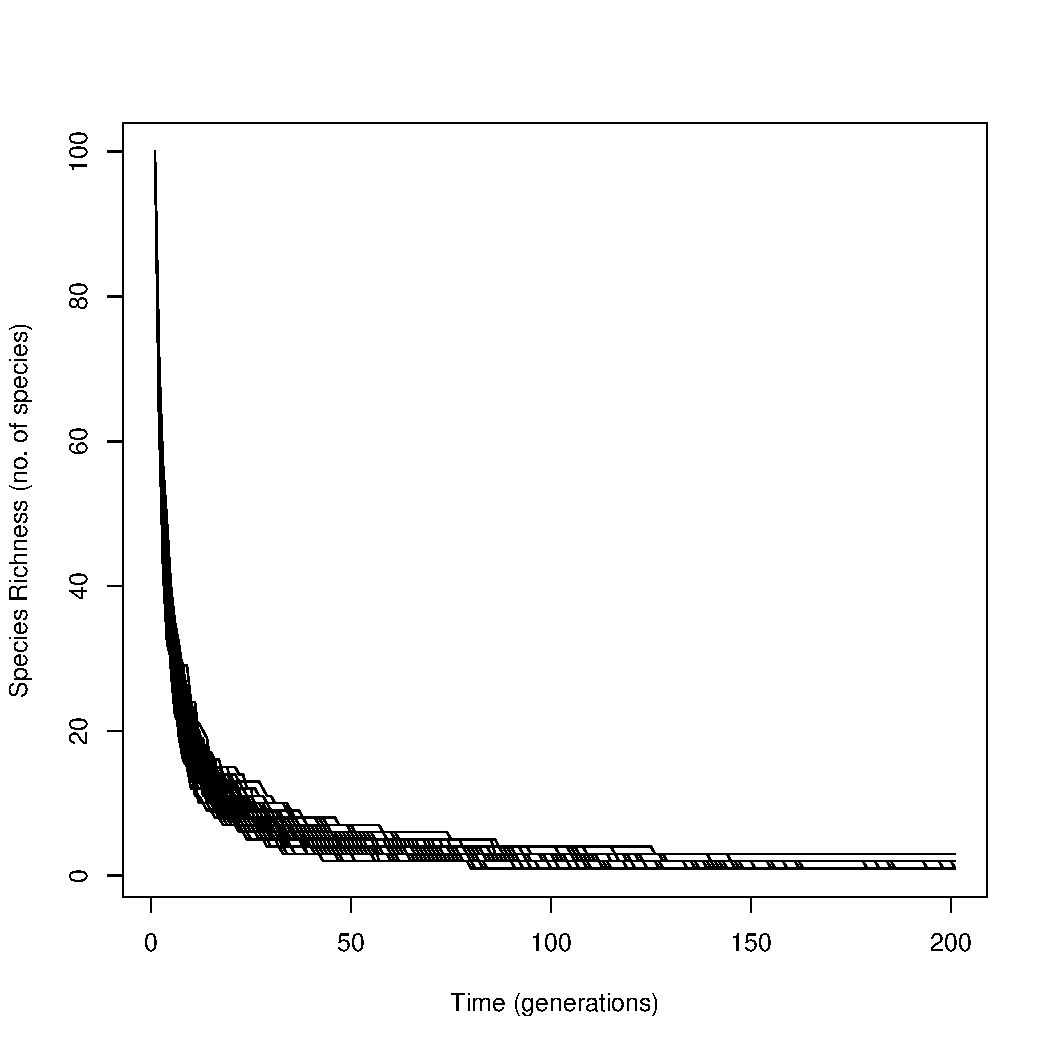
\includegraphics[width=\linewidth]{../Results/time_series2.pdf}
				\caption{}
			\end{subfigure}
			\caption{\textbf{(a)} Change in species richness over multiple generations. Initial community n = 100, with maximum species richness (all members of community different, 100 species). Simulation run over 200 generations, where a generation is defined by loss and replacement of half the community. \textbf{(b)} Simulation with same conditions but run over 100 iterations to show different scenarios.}
			\label{fig:qu8}
	\end{figure}

\newpage
\paragraph{Question 12:}\

\noindent \newline The neutral model simulation shown in Figure \ref{fig:q12} shows how a community that initially has a maximum species richness (red) will reach an equilibrium at a much lower species richness over time. The other community starts with a minimum species richness (blue) and with the effect of speciation, also reaches an equilibrium species richness, of a very similar level to the first community. This indicates, with the parameters used, communities are not dependent on their starting conditions when speciation occurs. In contrast to question 8, the model without speciation, this model shows speciation allows a higher equilibrium value of species richness, so several species becoming dominant within the community as opposed to a single species. When species richness drops within a community, this model assumes that there will be more of each species as community size is constant, therefore the lower the species richness, the larger the populations of each species, therefore the more resilient they are to extinction, which could explain the higher equilibrium value. \newline

		\begin{figure}[H]
			\centering
			\textbf{Neutral model simulation, with speciation, over 200 generations}\par\medskip
		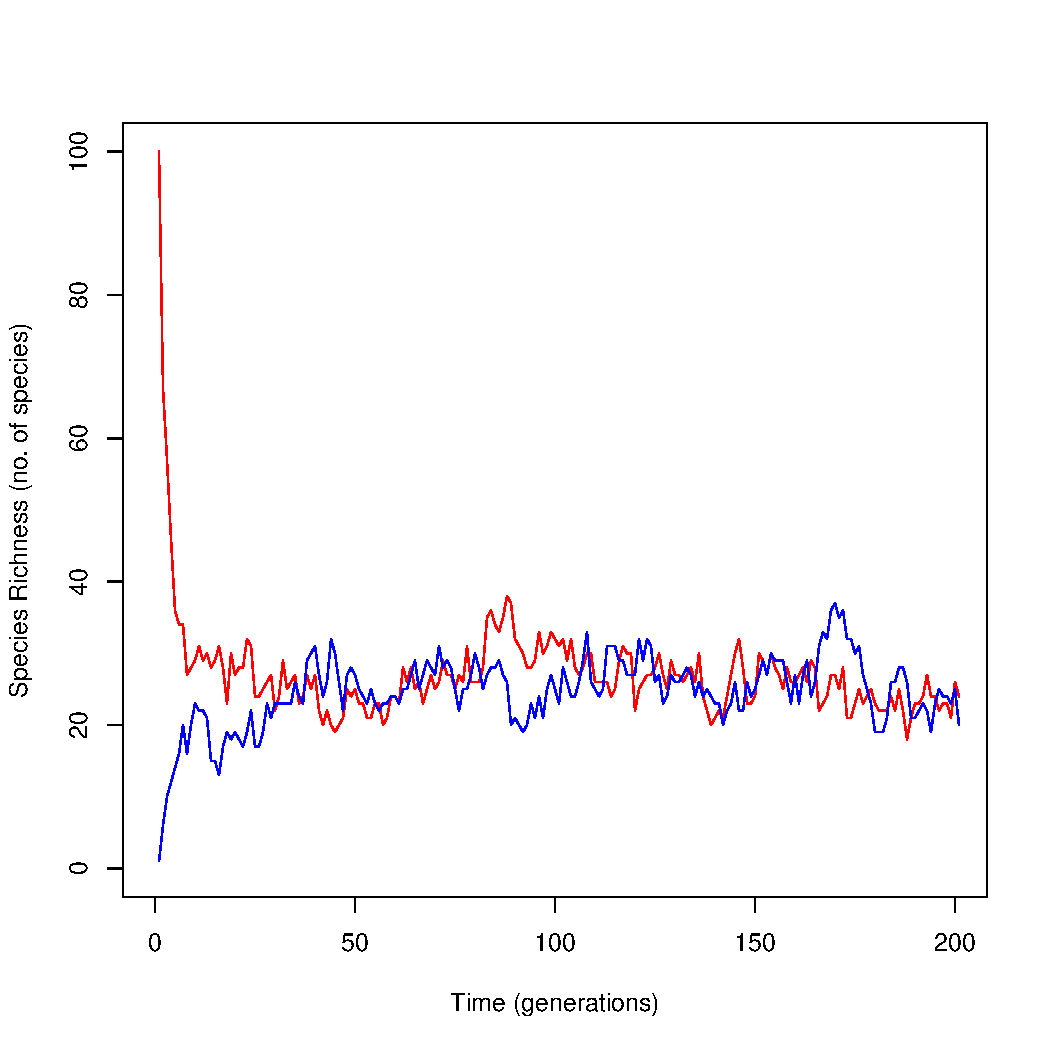
\includegraphics[width=0.8\linewidth]{../Results/time_series_speciation.pdf}
		\caption{Simulation of change in species richness of two communities, both with a 100 individuals, over 200 generations, with a speciation rate 0.2. The red community start with maximum and the blue start with minimum species richness.}
		% label invisible but can be used to refer to figure in text
		\label{fig:q12}
	\end{figure}

\newpage

\paragraph{Question 16:}\

\noindent \newline The initial condition of the system does not effect average abundances as the community stabilises by the end of the 200 generation burn out period, therefore does not effect the averaged abundances. As before, when the size of a single species gets smaller, the others in the constant size community grow to fill the space, leading to the majority of species having a low abundance and several dominant species having a higher abundance within the community, as shown in Figure \ref{fig:q16}.  \newline

	\begin{figure}[H]
	\centering
	\textbf{Neutral model simulation, with speciation, over 2000 generations}\par\medskip
	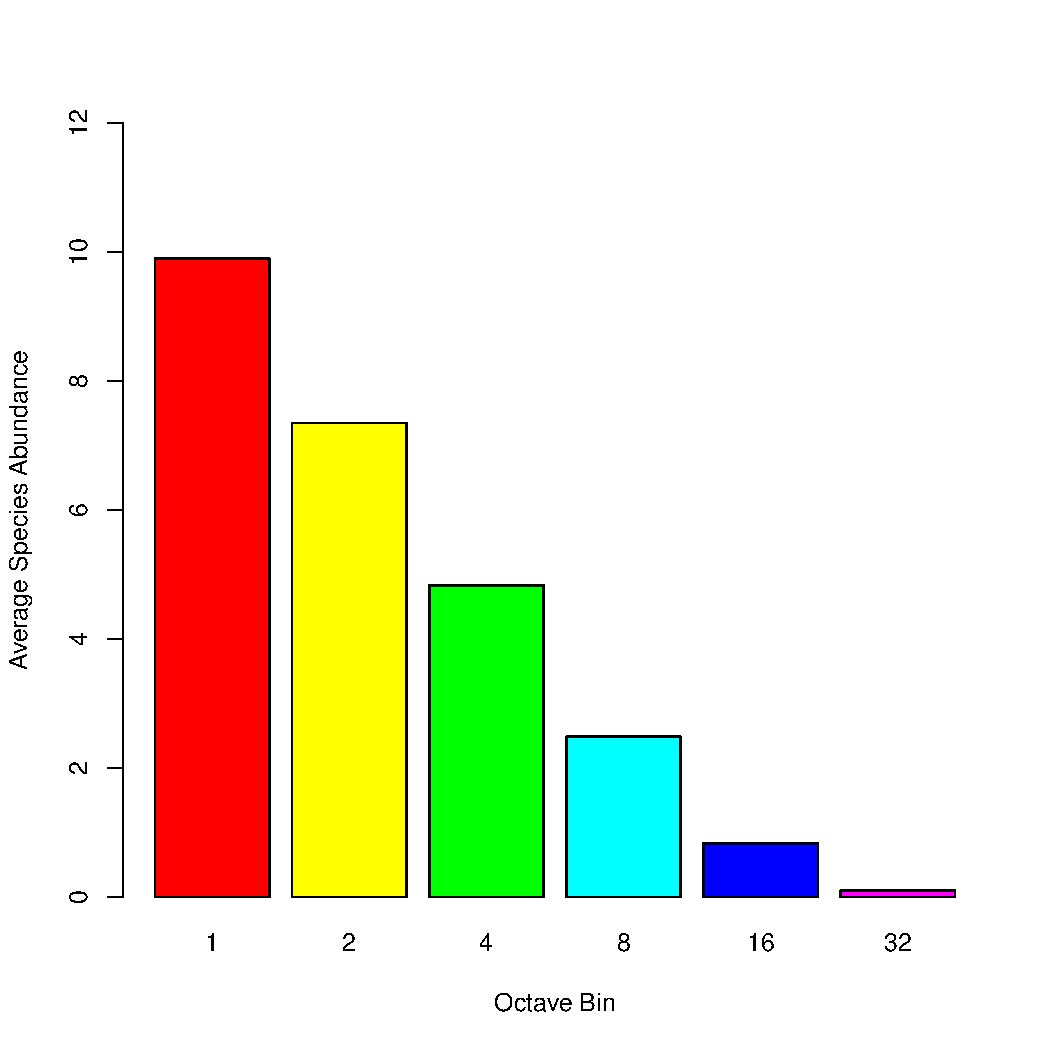
\includegraphics[width=0.8\linewidth]{../Results/octave_plot.pdf}
	\caption{Average of species abundance per octave bin, indicating that most species have a low abundance, and most have a high. Averaged from 101 values, from every 20th generation of a 2000 generation simulation (with a 200 generation burn in period), on a community of size 100.}
	% label invisible but can be used to refer to figure in text
	\label{fig:q16}
	\end{figure}

\newpage
\paragraph{Question 20:}\

\begin{figure}[H]
	\centering
	\textbf{Neutral model simulation with communities of 500,1000,2500 and 5000, \\ speciation rate of 0.004686}\par\medskip
	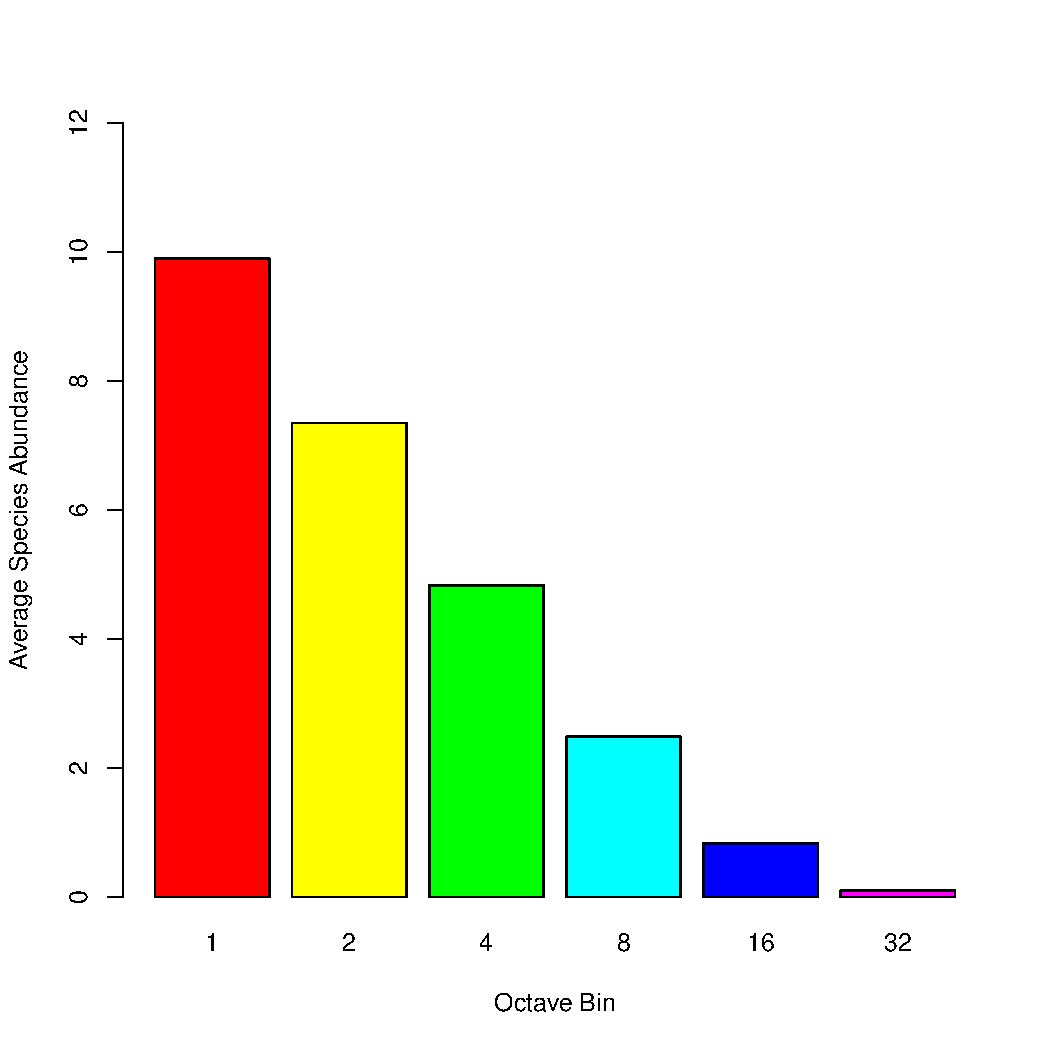
\includegraphics[width=\linewidth]{../Results/octave_plot.pdf}
	\caption{THIS IS NOT THE CORRECT FIGURE FOR THIS QUESTION, WILL BE CHANGED BY 5PM TUESDAY. Mean species abundance for each octave. Simulated using neutral theory, over a period of 11.5 hours using HPC, and communities of \textbf{(a)} 500, \textbf{(b)} 1000, \textbf{(c)} 2500 and \textbf{(d)} 5000, each run 25 times. Simulation used a speciation rate of 0.004686, a burn in period of 8 x respective community size, number of generations were community size divided by 10. The abundances generated were collected into octaves and averaged across each community.}
	% label invisible but can be used to refer to figure in text
	\label{fig:q20}
\end{figure}

\newpage
\paragraph{Question 21:}\

\noindent \newline The fractal dimensions of the two objects shown in Figure \ref{fig:qu21} were calculated using the law that the fractal dimension D = log(n)/log(r) where r is the scale factor between length of the original fractal shape and the new fractal shape and n is the number of repeats of the original shape that make up the new. In the case of Sierpinski's carpet, Figure \ref{fig:qu21}a, the r value is 3 as a smaller unit is repeated in length 3 times to make up the larger, and n = 8 as 8 of the original fractal repeat to make the new, therefore D = 1.89. Menger's sponge, Figure \ref{fig:qu21}b, again has an r value of 3, and the n = 20, as 20 smaller cubes make up the larger, giving a fractal dimension D = 2.73.

	\begin{figure}[H]
		\centering
		\begin{subfigure}[t]{0.37\linewidth}
			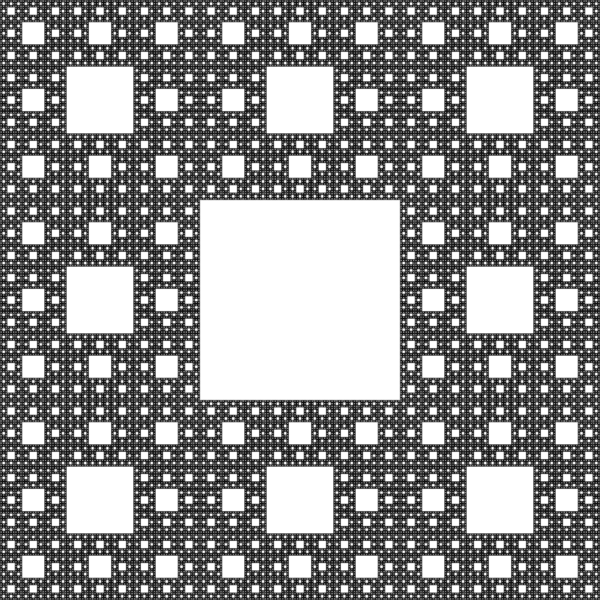
\includegraphics[width=\linewidth]{../Data/Sierpinski_carpet.jpg}
			\caption{}
		\end{subfigure}
		\begin{subfigure}[t]{0.5\linewidth}
			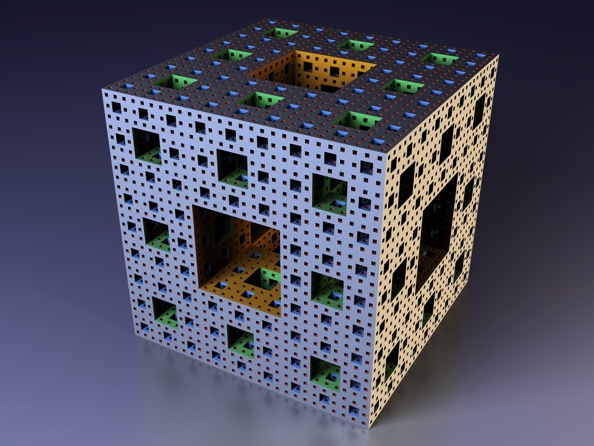
\includegraphics[width=\linewidth]{../Data/menger_sponge.jpg}
			\caption{}
		\end{subfigure}
		\caption{\textbf{(a)} Sierpinski's carpet and \textbf{(b)} Menger's sponge.}
		\label{fig:qu21} 
	\end{figure}

\paragraph{Question 22:}\

\noindent \newline The code used to create the chaos game function plots a transformed version of Sierpinski's Gasket.

\paragraph{Question 25:}\

\noindent \newline As the function is required to call itself, it has no end point, therefore will plot infinitely. This will cause an error as it effectively runs forever.

\newpage
\paragraph{Question 26:}\

\noindent \newline This spiral function works as an end point is set, gives Figure \ref{fig:q26}.

\begin{figure}[H]
	\centering
	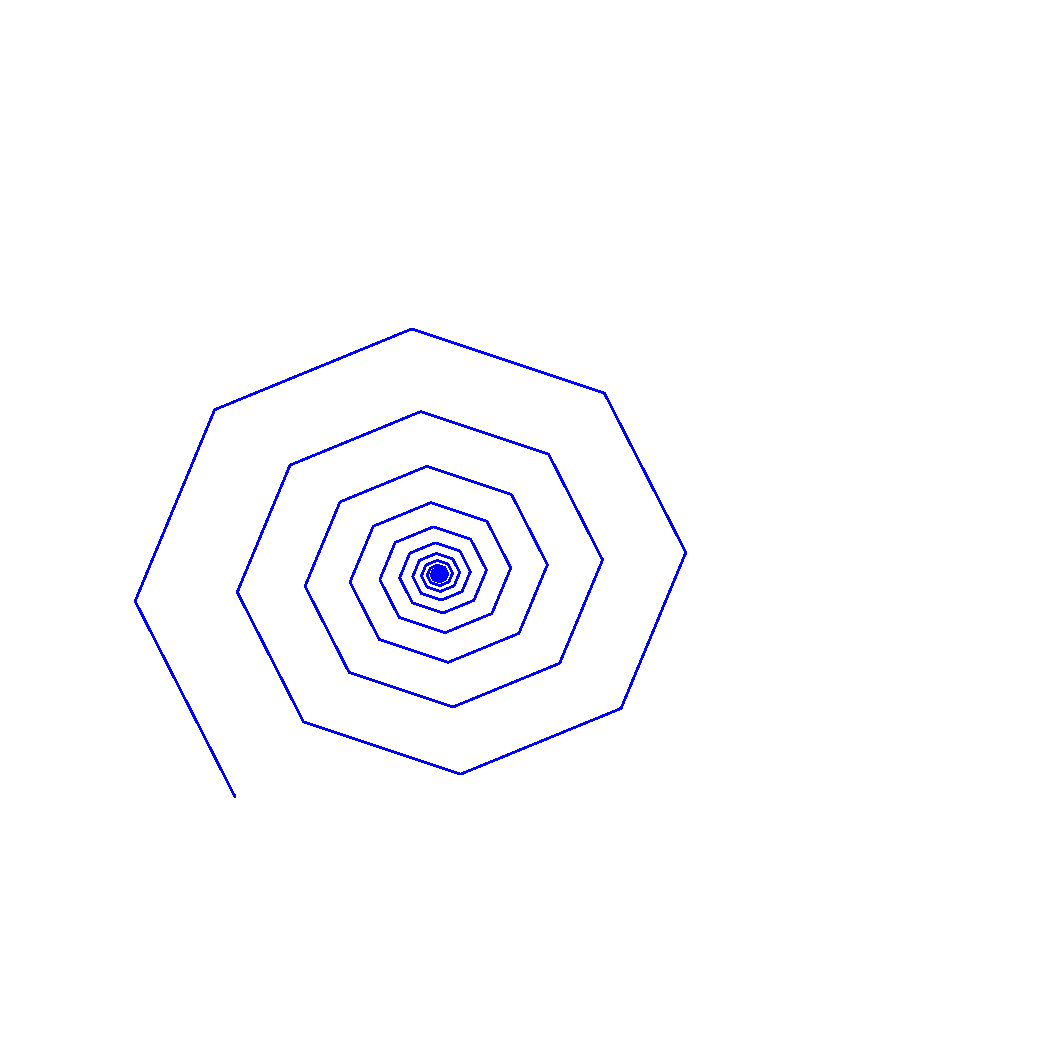
\includegraphics[width=0.5\linewidth,trim={2cm 3cm 6cm 5cm},clip]{../Results/spiral_2.pdf}
	\caption{Using spiral function with end point.}
	% label invisible but can be used to refer to figure in text
	\label{fig:q26}
\end{figure}

\paragraph{Question 27:}\

\begin{figure}[H]
	\centering
	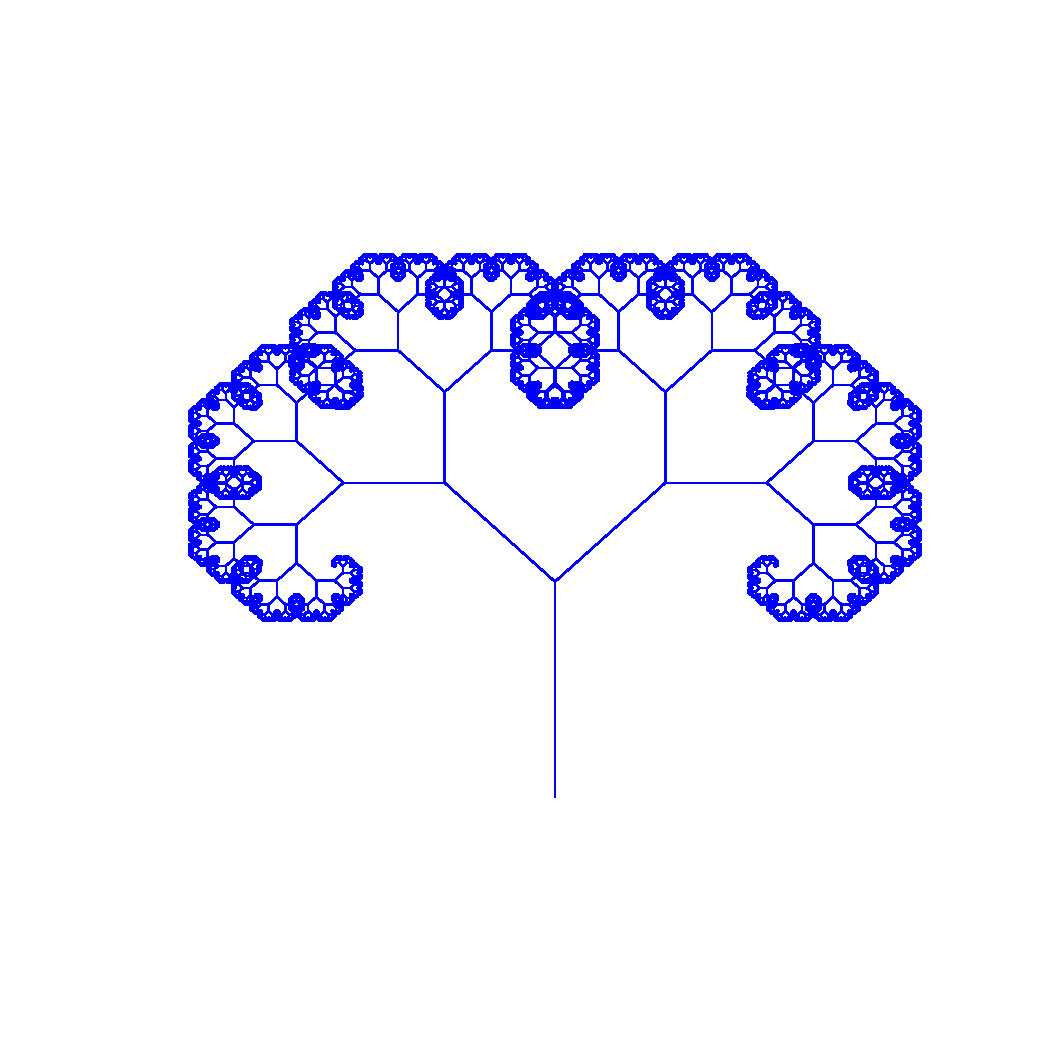
\includegraphics[width=0.5\linewidth,trim={3cm 3cm 2cm 2cm},clip]{../Results/tree.pdf}
	\caption{Using an adapted version of the function used to draw Figure \ref{fig:q26} to draw a tree.}
	% label invisible but can be used to refer to figure in text
	\label{fig:q27}
\end{figure}

\newpage

\paragraph{Question 29:}\	


\begin{figure}[H]
	\centering
	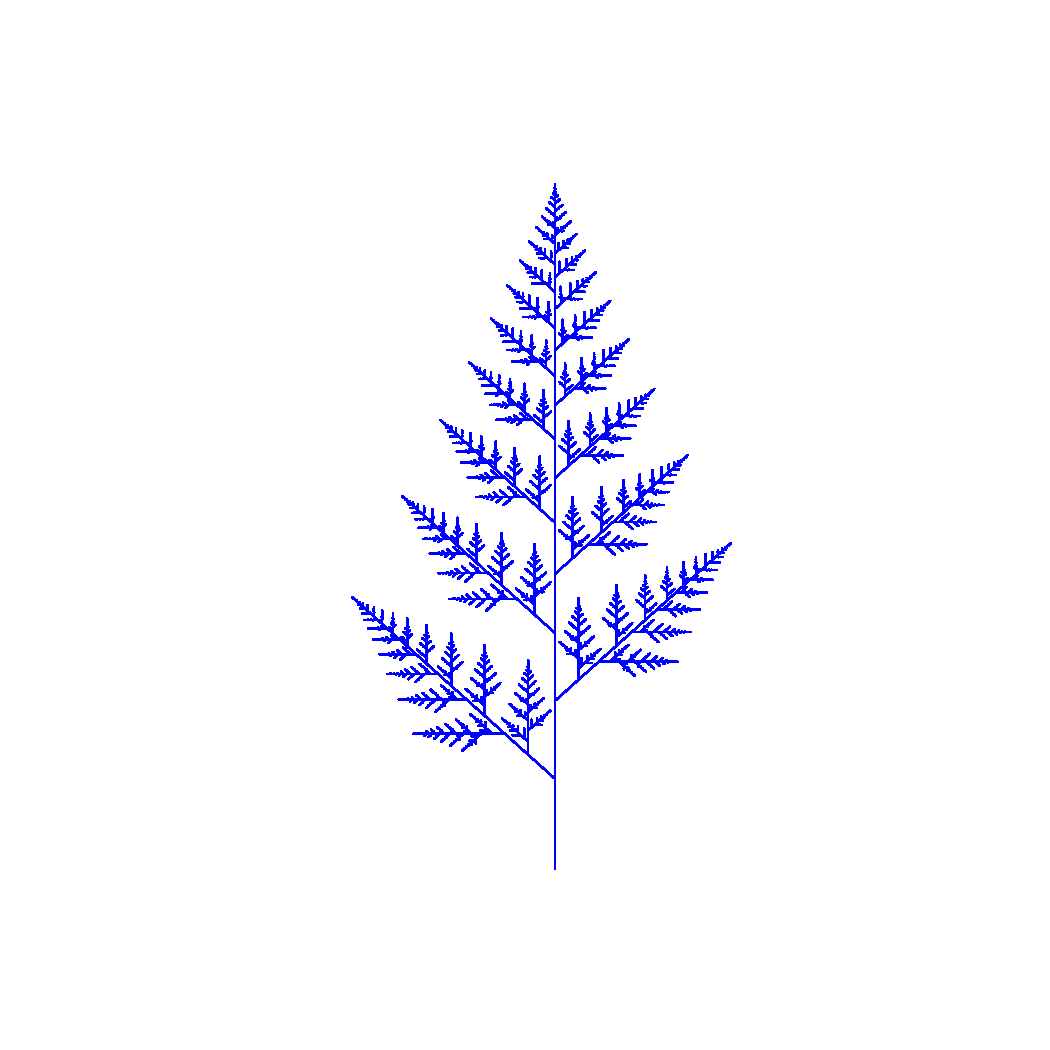
\includegraphics[width=0.5\linewidth,trim={3cm 3cm 2cm 2cm},clip]{../Results/fern_2.pdf}
	\caption{Fern drawn using a code adapted from the tree function shown in Figure \ref{fig:q27}.}
	% label invisible but can be used to refer to figure in text
	\label{fig:q29}
\end{figure}

\newpage
\section*{HPC Challenge Question Written Answers}
 
\paragraph{Challenge Question E:}\

\noindent \newline Changing the starting point of the chaos game function does not effect the output, giving the same image each time. When the points of the function are set to an equilateral triangle, the function produces Sierpinski's Gasket, Figure \ref{fig:E}.

\begin{figure}[H]
	\centering
	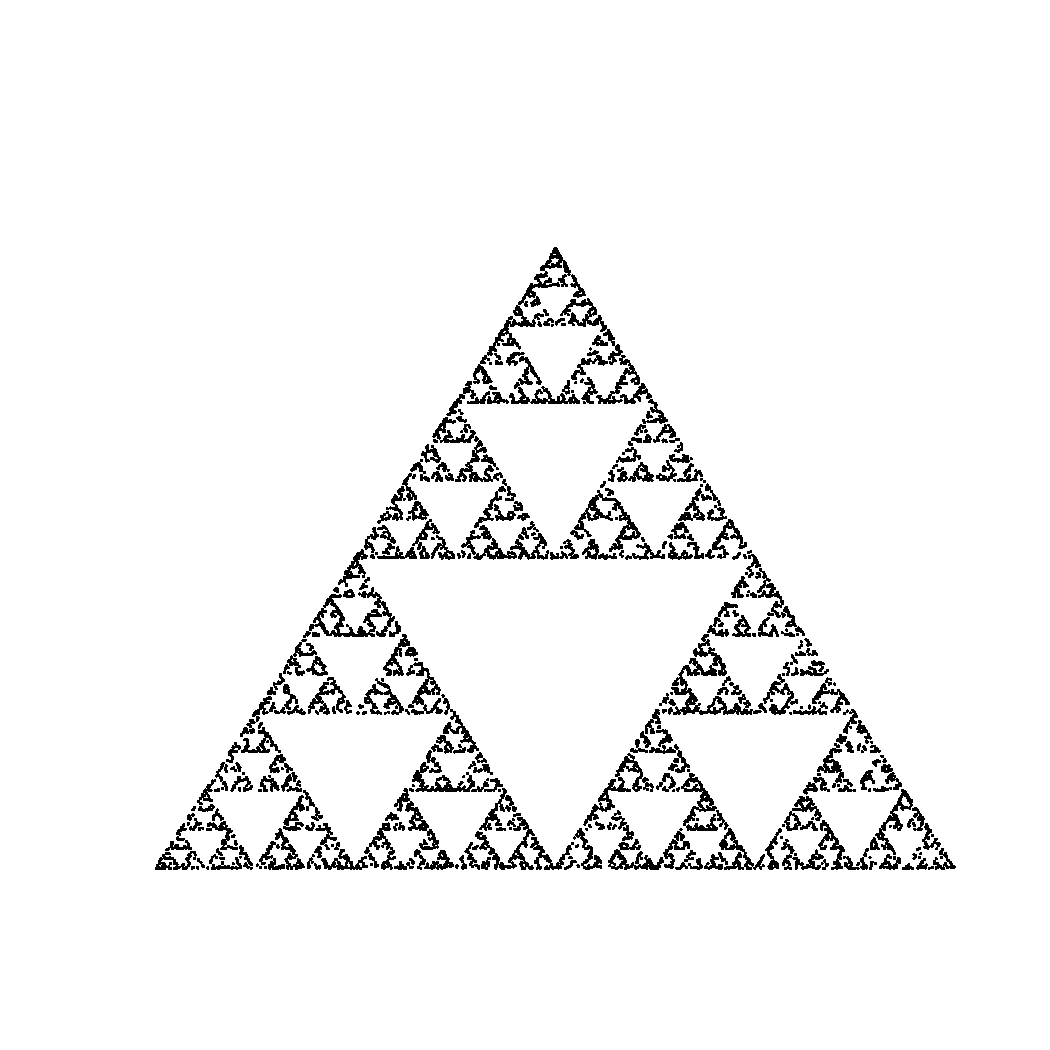
\includegraphics[width=0.5\linewidth,trim={1cm 1cm 1cm 1cm},clip]{../Results/s_gasket.pdf}
	\caption{Sierpinski's gasket using an equilateral form of the chaos game function.}
	% label invisible but can be used to refer to figure in text
	\label{fig:E}
\end{figure}

	
\end{document}